\chapter{Introduction} \label{ch:introduction}

Digifiz Replica and Digifiz Replica Next are retrofit digital instrument clusters designed for Volkswagen Golf Mk2, Jetta Mk2, and Scirocco Mk2 vehicles.
The dashboards replace the factory analogue panel while adding fully digital readouts, multi-function (MFA) trip computation, support for both cable and electronic speed sensors, and remote configuration interfaces.
This manual combines the information required to identify the available hardware variants, install the cluster, operate the MFA features, and maintain both generations of the product.

The document is organised so that each chapter focuses on one aspect of the system: product identification and connector pin-outs, operating principles and environmental limits, installation and everyday use, configuration of the Replica Next Wi-Fi interface, Bluetooth-based configuration for the classic Replica, troubleshooting guides, and the rules for labelling, packaging, and storage.
Readers who are preparing to install the instrument cluster for the first time should start with \Cref{ch:description,ch:preparation}, while experienced users will find configuration references in \Cref{ch:replica-next-setup,ch:replica-setup}.

\begin{figure}[htbp]
    \centering
    \begin{subfigure}{0.48\textwidth}
        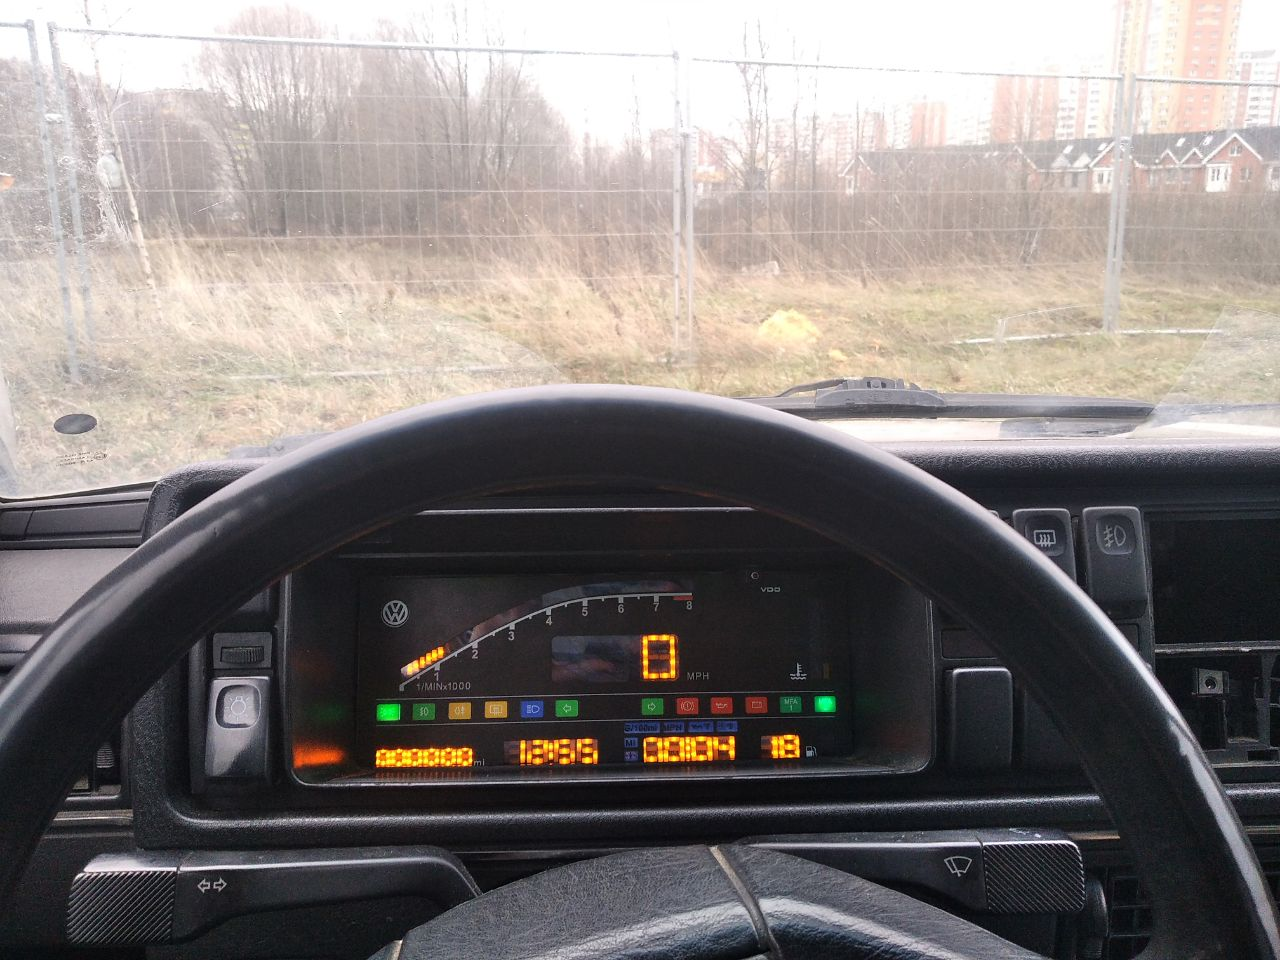
\includegraphics[width=\linewidth]{digifiz_manual/image004.jpg}
        \caption{Digifiz Replica Next powered on in the vehicle cockpit.}
    \end{subfigure}\hfill
    \begin{subfigure}{0.48\textwidth}
        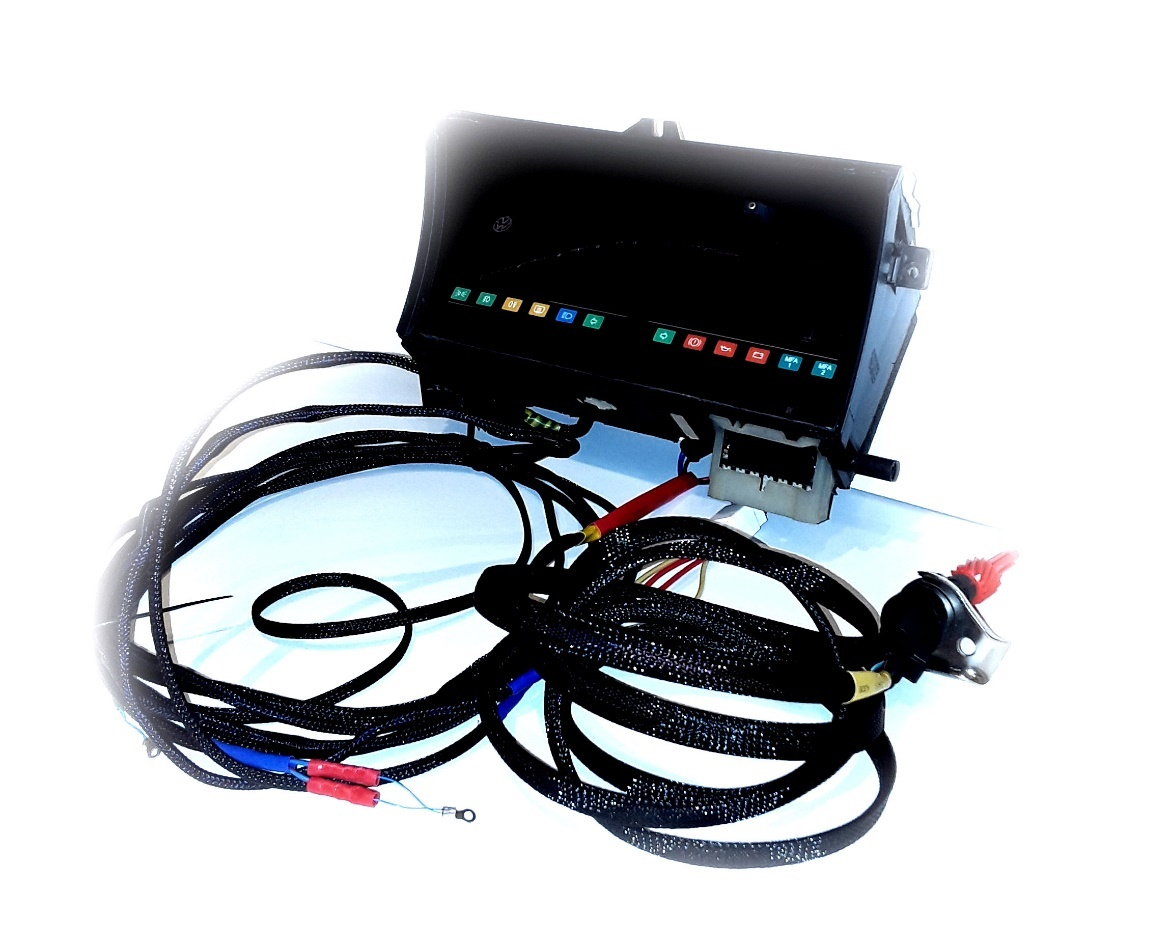
\includegraphics[width=\linewidth]{digifiz_manual/image005.jpg}
        \caption{Replica Next delivery set (GART 8--MGF variant).}
    \end{subfigure}
    \begin{subfigure}{0.48\textwidth}
        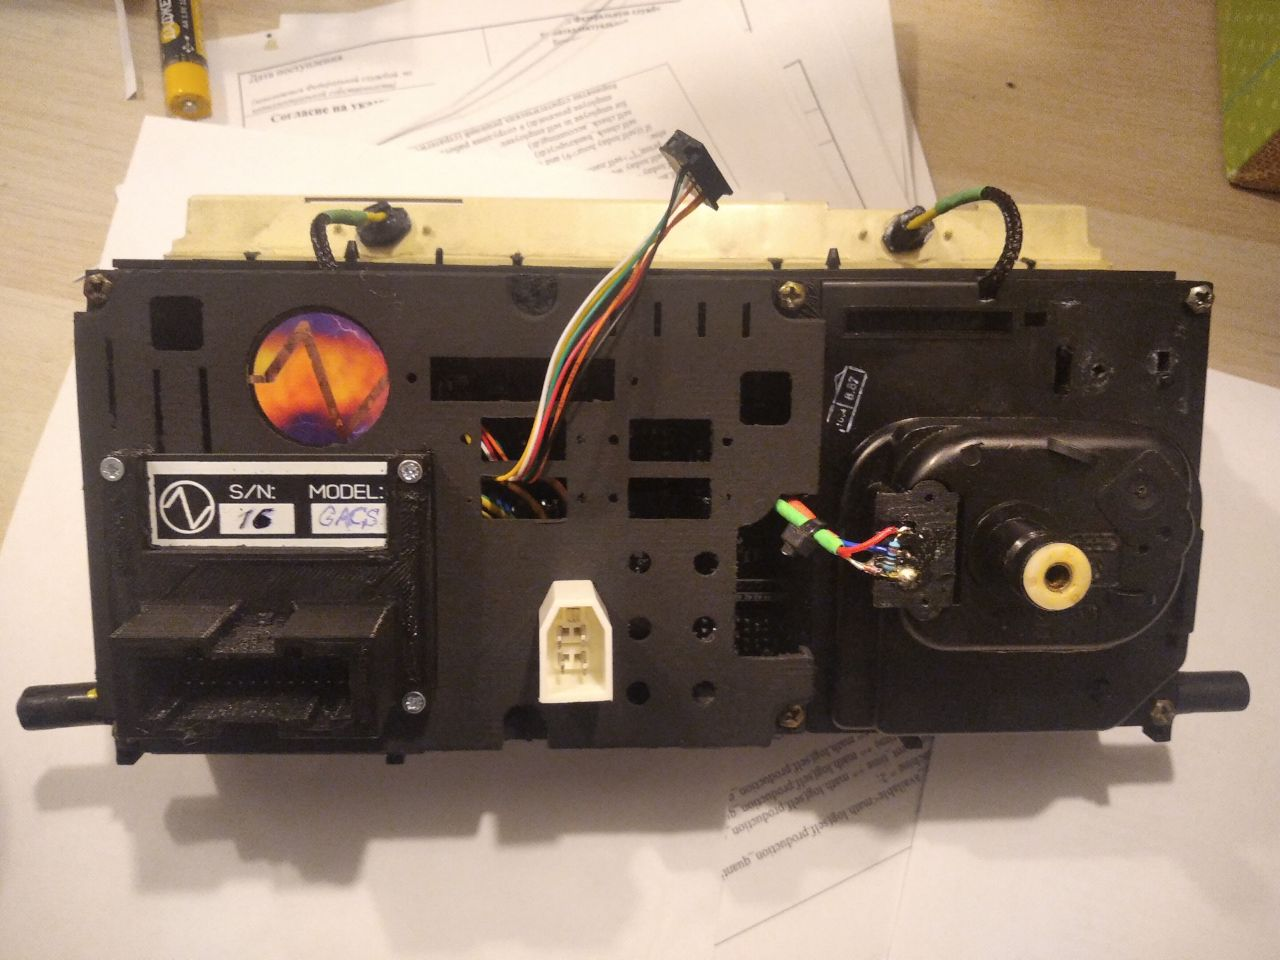
\includegraphics[width=\linewidth]{digifiz_manual/image006.jpg}
        \caption{Rear view of a single-connector (GACS) assembly.}
    \end{subfigure}\hfill
    \begin{subfigure}{0.48\textwidth}
        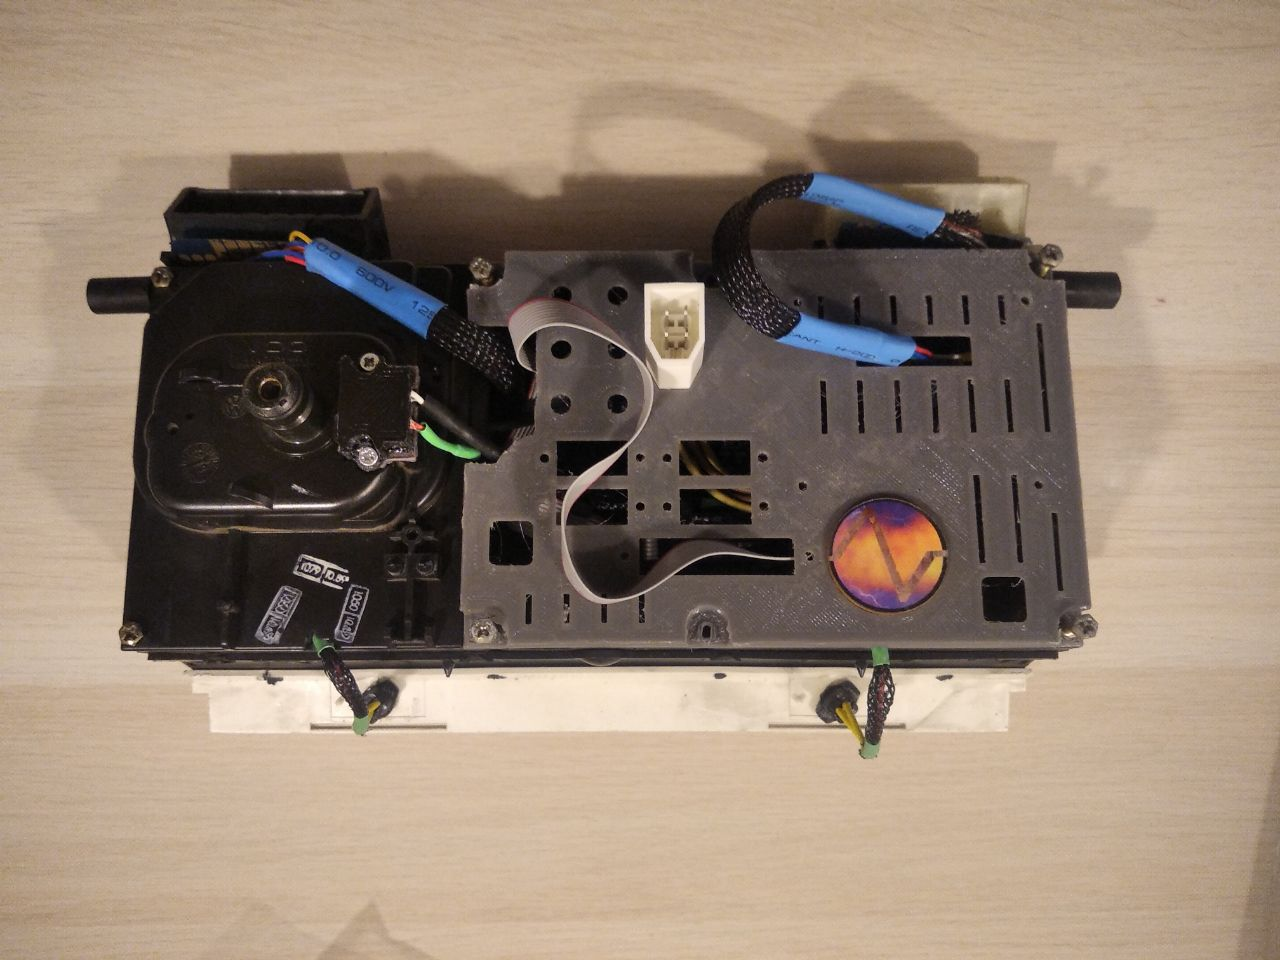
\includegraphics[width=\linewidth]{digifiz_manual/image007.jpg}
        \caption{Rear view of a dual-connector (GACT) assembly.}
    \end{subfigure}
    \caption{Representative Digifiz Replica instrument cluster configurations.}
    \label{fig:intro-product-views}
\end{figure}

The Replica family is supplied in several configurations to match petrol and diesel drivetrains, left-hand and right-hand drive harnesses, and regional measurement units.
Later chapters describe the coding scheme in detail and provide tables for each connector so that the cluster can be installed safely without factory documentation.
